\section{Ansteuerung}
\label{kap:Ansteuerung}
Der Aufbau des Gesamtsystem und dessen Funktionsweise ist in Abbildung \ref{fig:aufbau} prinzipiell dargestellt.
Dabei ist zun�chst das mechanische Modell vernachl�ssigbar, da dieses im weiteren Verlauf Erl�uterung findet. Zun�chst wird die softwaretechnische Seite betrachtet und dessen elektronischen Komponenten, die zur Ansteuerung des Gesamtsystems genutzt werden, erl�utert.

\begin{figure}[H]
\centering
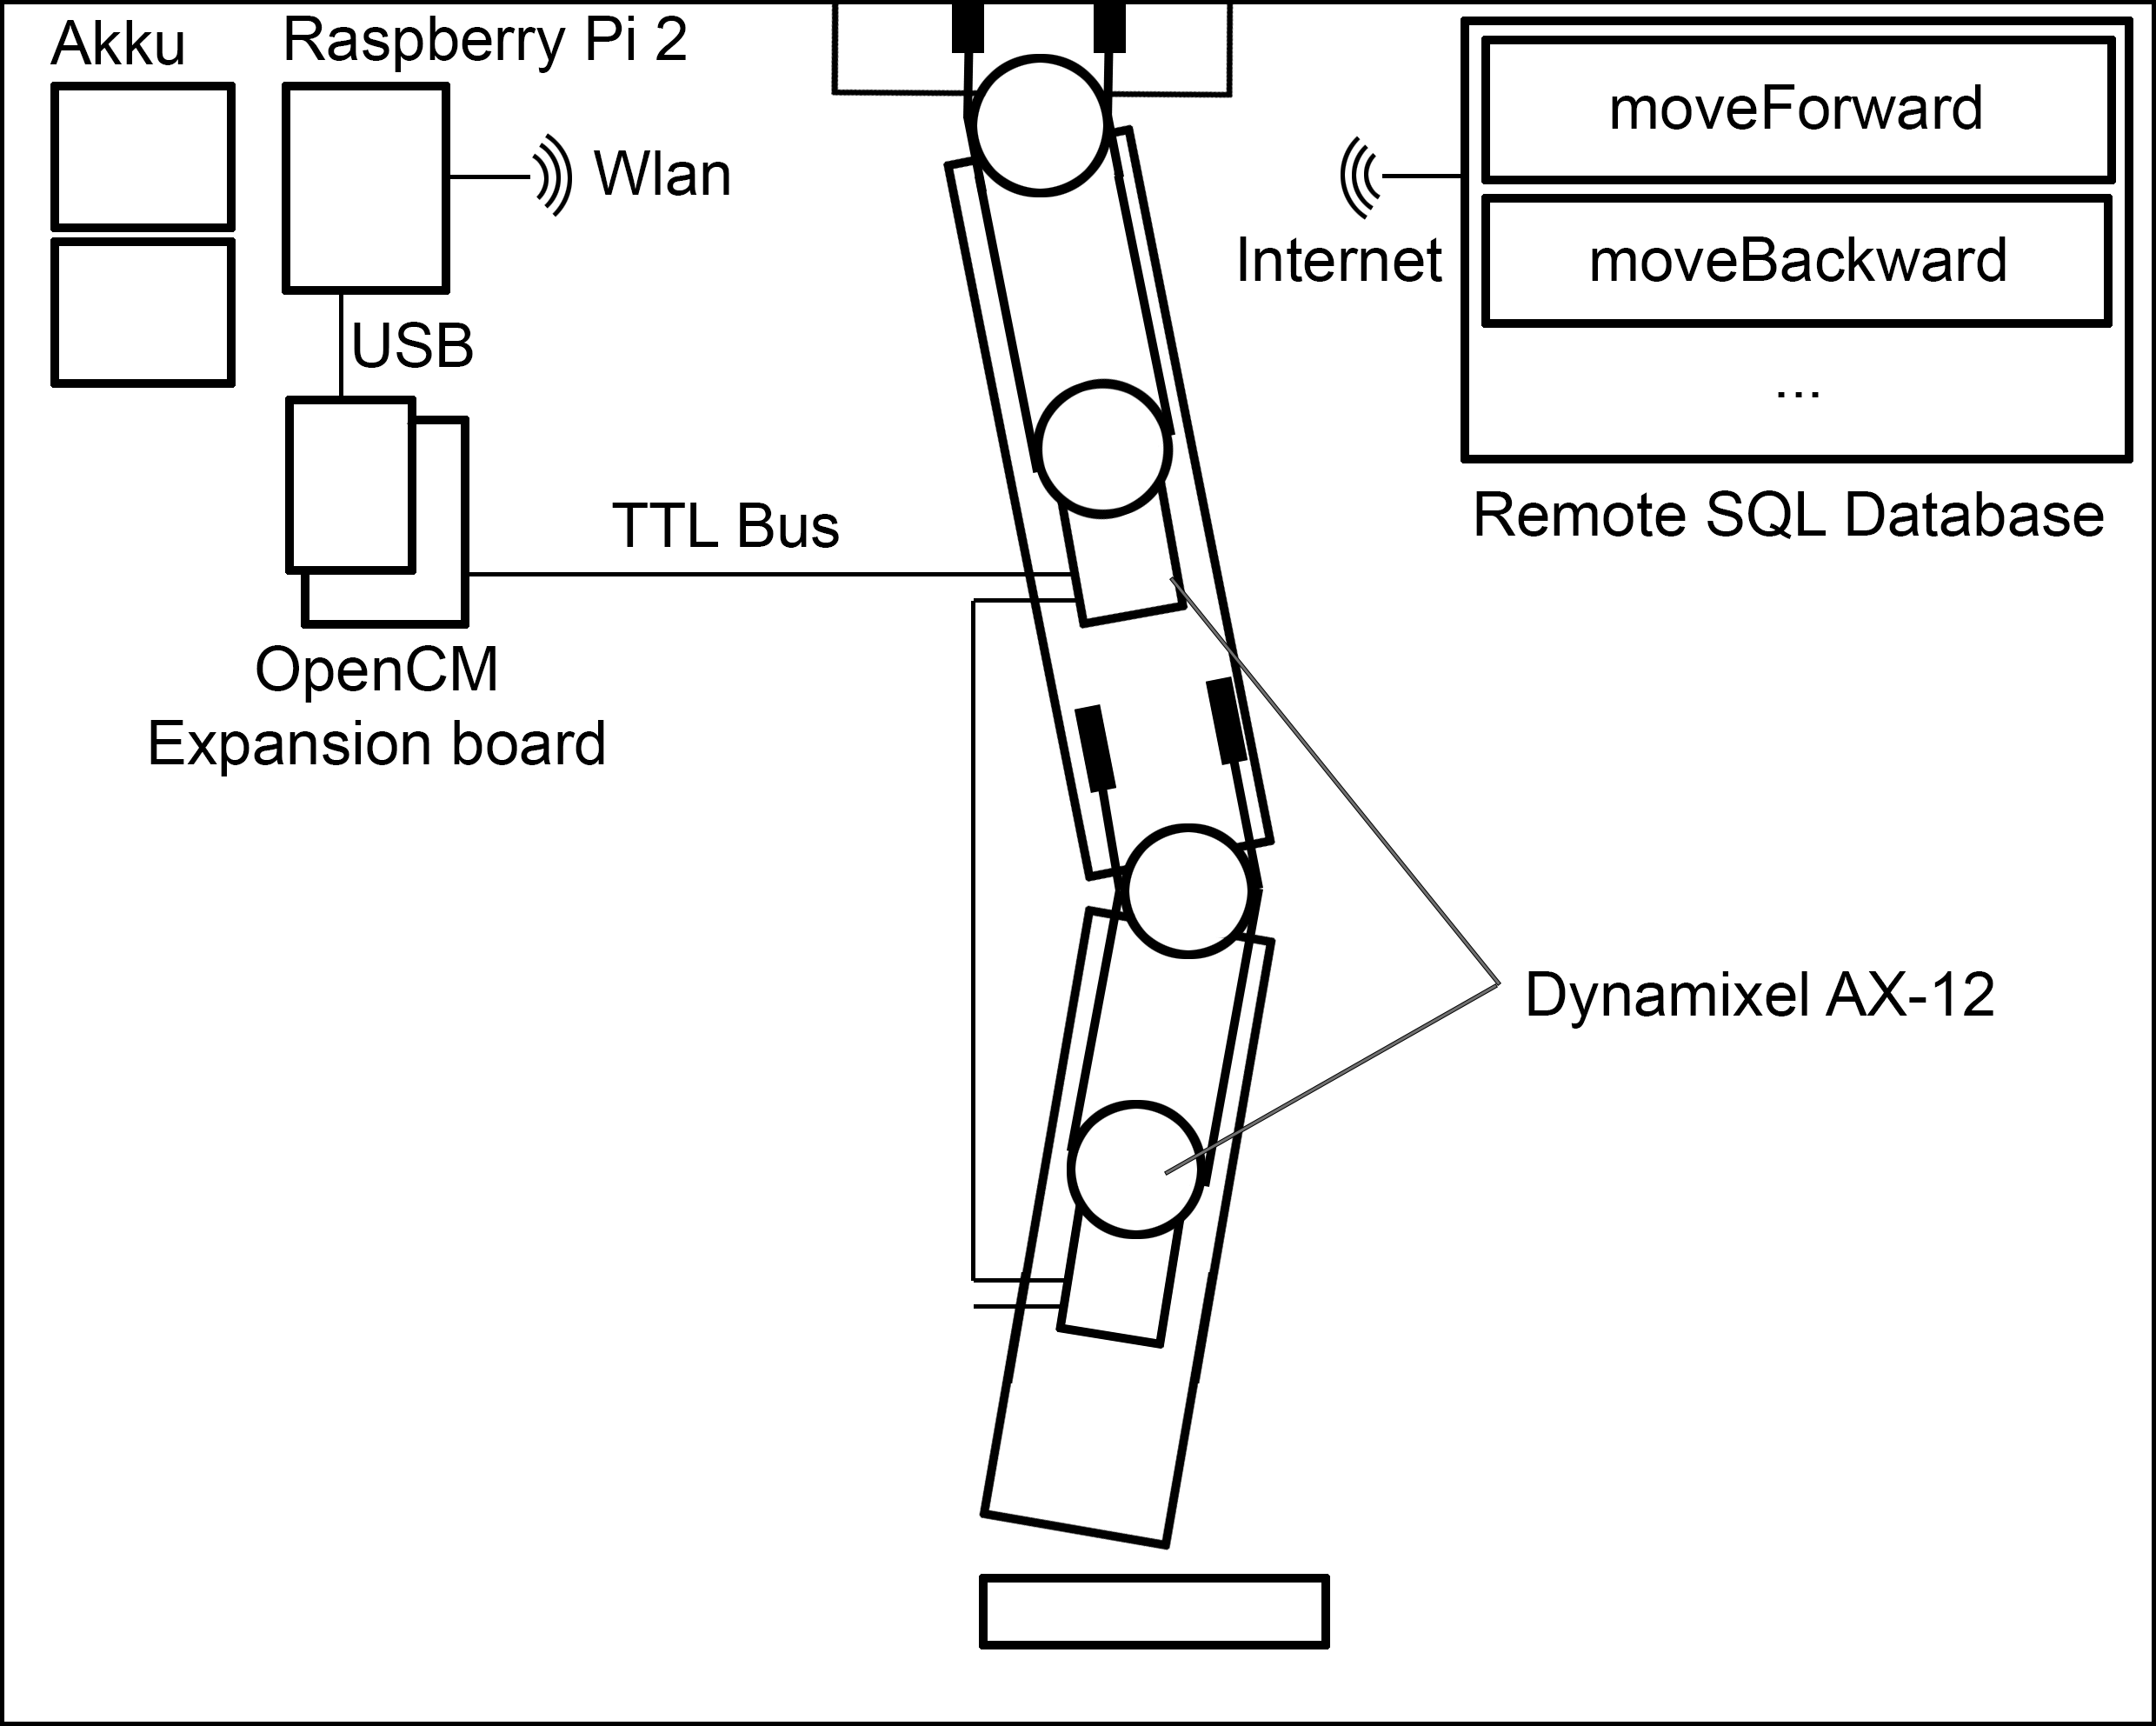
\includegraphics[width=1.0\linewidth]{03_Grafiken/Robotersystem/Aufbau}
\caption[Ansteuerung / Aufbau (Prinzip)]{Ansteuerung / Aufbau (Prinzip)}
\label{fig:aufbau}
\end{figure}

Diesbez�glich befindet sich im oberen linken Teil der Grafik die Konstellation der beteiligten Baugruppen und deren Verkn�pfung zueinander. Der Raspberry Pi 2 dient als Steuerzentrale, auf dem das \gls{BS} Windows 10 IOT installiert ist. Darauf ist eine Software aktiv, mit der die gesamte Reglung des Systems abgearbeitet wird. Entsprechend erfolgt das Senden von Befehlen (zur Ansteuerung der Motoren) vom Raspberry Pi aus �ber eine USB-Schnittstelle hin zum OpenCM Board. Dieses Board liest die Befehle und gibt diese an die Motoren (Dynamixel AX-12) weiter. Das Expansion Board ist notwendig, da das OpenCM-Board keine TTL-Schnittstelle zur Verf�gung stellt.\\
Der eigentlich Clou des Systems besteht darin, dass beim Neustart (sofern notwendig) die Bewegungss�tze von einer externen Datenbank heruntergeladen werden. Diesbez�glich verf�gt der Raspberry Pi �ber eine Wlan, bzw. UMTS-Schnittstelle. Die SQL-Datenbank ist �ber das Internet erreichbar, sodass stets aktuelle Bewegungss�tze zur Verf�gung stehen. Die Bewegungss�tze werden mit dem, in Kapitel \ref{kap:Messsystem} beschriebenen Messsystem erstellt / erweitert.
\subsection{Protokoll}
\label{kap:Protokoll}
Sobald auf dem Raspberry Pi die gesamten Bewegungss�tze zur Verf�gung stehen, beginnt der Kontrollalgorithmus und navigiert den Roboter, entsprechend der Eingangsgr��en (visuell, haptisch, etc.). Dazu kommt ein �bertragungsprotkoll zum Tragen, welches (in der aktuellen Version) das Ansteuern von 8 Motoren gleichzeitig zul�sst. Das Protokoll (s. Abbildung \ref{fig:protokoll}) darf 64 byte nicht �berschreiten, da dies die maximale Menge ist, die per Sequenz �ber die USB-Schnittstelle des OpenCM-Boards �bertragen werden kann. 

\begin{figure}[H]
\centering
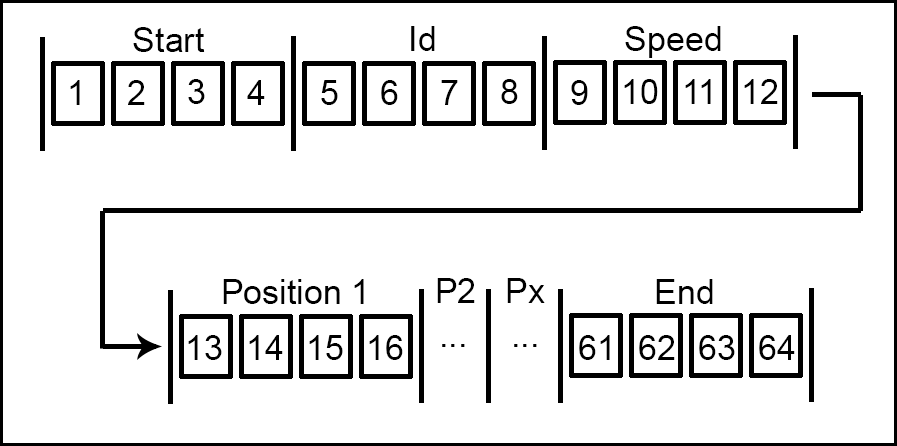
\includegraphics[width=0.7\linewidth]{03_Grafiken/Robotersystem/Protokoll}
\caption[�bertragungsprotkoll]{�bertragungsprotkoll}
\label{fig:protokoll}
\end{figure}

Die �bertragung der Stellgr��en, f�r acht Motoren per Zyklus, erfolgt blockweise mit einer Blockgr��e von 2 byte. In der obigen Grafik ist der Inhalt jedes Blocks dargestellt. Beginnend mit der Startsequenz (Dezimalwert: 9999), folgen die IDs der Motoren (bitweise: ...0000 0001, jedes Bit repr�sentiert einen Motor: 1 aktiv, 0 inaktiv). Insgesamt k�nnen 14 Motoren per Sequenz angesprochen werden. Nach dem Block der IDs folgt die Geschwindigkeit mit der die Positionen angefahren werden sollen. Diese sind nacheinander f�r jeden Motor mit jeweils 2 byte definiert (14 Motoren a 2 byte = 28 byte). Nach den Geschwindigkeiten sind die Bl�cke f�r die Positionen angeordnet. Diese sind ebenfalls f�r jede Position nacheinander mit jeweils 2 byte definiert. Das Ende einer Nachricht wird mit der Endsequenz angegeben (Dezimal: 8888);

\subsection{Testprogramm}
% WriteToComPort

\subsection{Kontrollprogramm}
% MovementControl

\subsection{Clientprogramm}
% Programm auf dem OpenCM